\documentclass[a4paper]{amsart}            %for bookmarks enable option [liststotoc]%



%-------packages-------------------------%

%Languages: Uncomment for German Package:
%\usepackage[latin1]{inputenc}
%\usepackage[T1]{fontenc} 
%\usepackage[ngerman]{babel} 

\usepackage{amsmath}
\usepackage{amsthm}        % Does theorem stuff
\usepackage{amssymb} 

%\usepackage{biblatex}
%\bibliography{over2}

\usepackage{scrextend}

\usepackage{tikz}
\usepackage{pgf}
\usetikzlibrary{calc, through, matrix, arrows,positioning, decorations.pathmorphing }

\usepackage[margin=1.5in]{geometry}

\usepackage{enumitem}

\usepackage{tikz}
\usetikzlibrary{%
  matrix,%
  calc,%
  arrows%
}

\usepackage{color}
\usepackage{hyperref}


\definecolor{matall-grey}{gray}{0.25}
\definecolor{darkblue}{rgb}{0.0,0.0,0.3}  

%pdf book marks the way I like%
\hypersetup{pdftex=true, colorlinks=true, breaklinks=true, linkcolor=darkblue, menucolor=darkblue, pagecolor=darkblue, urlcolor=darkblue}


%-----------style------------------------%


%----------new--commands-----------------%

\newcommand{\C}{\mathcal{C}}
\renewcommand{\O}{\mathcal{O}}
\newcommand{\D}{\mathcal{D}}
\newcommand{\F}{\mathcal{F}}
\newcommand{\G}{\mathcal{G}}
\newcommand{\ve}{\varepsilon}
\newcommand{\Mor}{\mathrm{Mor}}
\newcommand{\id}{\operatorname{id}}
\newcommand{\Hom}{\operatorname{Hom}}
\newcommand{\Z}{\mathbb{Z}}
\newcommand{\N}{\mathbb{N}}

% --- homology ---- %
\newcommand{\HCW}[1]{\widetilde{H}^{\operatorname{CW}}_{#1}}
\newcommand{\Hred}[1]{\widetilde{H}_{#1}}
\newcommand{\CWchain}[1]{\widetilde{C}^{\operatorname{CW}}_{#1}}
\newcommand{\dCW}[1]{d^{\operatorname{CW}}_{#1}}

\DeclareMathOperator{\coker}{coker}
\DeclareMathOperator{\im}{im}
\DeclareMathOperator{\tr}{tr}






 
    
  

\newenvironment{tmo}[1]{%
  \trivlist
  \leftskip=0.15cm
  \item[\hskip\labelsep
        \bfseries
   #1\@{.}]\mbox{ }\par\nobreak
   \vskip -0.5em\nobreak% Absatzabstand nachträglich entfernen.
   \noindent
  \leftskip=0.35cm
  \rightskip=0.35cm
  \itshape\ignorespaces
}{%
\endtrivlist}

\newcounter{tm}
% Falls tm abhängig von \section nummeriert werden soll:
%\numberwithin{tm}{section}% anderenfalls auskommentieren!!!
\newenvironment{tm}[1]{% wie tmo aber mit Nummer
  \refstepcounter{tm}%
  \tmo{#1~\thetm}%
}{%
  \endtmo
}
     
\makeatletter
\renewenvironment{proof}[1][\proofname]{\par
  \pushQED{\qed}%
  \normalfont \topsep6\p@\@plus6\p@\relax
  \trivlist
  \leftskip=0.6cm
  
  \item[\hskip\labelsep
        \itshape
    #1\@addpunct{.}]\mbox{ }\par\noindent%
  \leftskip=1cm
  \rightskip=1cm    
}{%
  \popQED\endtrivlist\@endpefalse
}
\makeatother 

\theoremstyle{plain}                                               %%
 \newtheorem{theorem}[equation]{Theorem}                            %%
 \newtheorem*{claim}{Claim}                                         %%
 \newtheorem*{lemma*}{Lemma}
 \newtheorem*{proposition*}{Proposition}                                       %%
 \newtheorem*{theorem*}{Theorem}                                    %%
 \newtheorem{lemma}[equation]{Lemma}                                %%
 \newtheorem{corollary}[equation]{Corollary}                        %%
 \newtheorem{proposition}[equation]{Proposition}                    %%

%--produce-the-warning--symbol-----------%
 \DeclareFontFamily{U}{manual}{}                                
 \DeclareFontShape{U}{manual}{m}{n}{ <->  manfnt }{}            
 \newcommand{\manfntsymbol}[1]{%                                
    {\fontencoding{U}\fontfamily{manual}\selectfont\symbol{#1}}}

\makeatother


\begin{document}

%------------header----------------------%

\title{Quantum Mechanics}
%\author{Felix Hoffmann}% %for now I decided against it%


%\maketitle
\pagestyle{empty} %no pagenumbers and titles%
\thispagestyle{empty}

\abovedisplayskip\smallskipamount
\belowdisplayskip \abovedisplayskip
%-------end header-----------------------%


\begin{center}
%\resizebox{11.5cm}{!}{%
	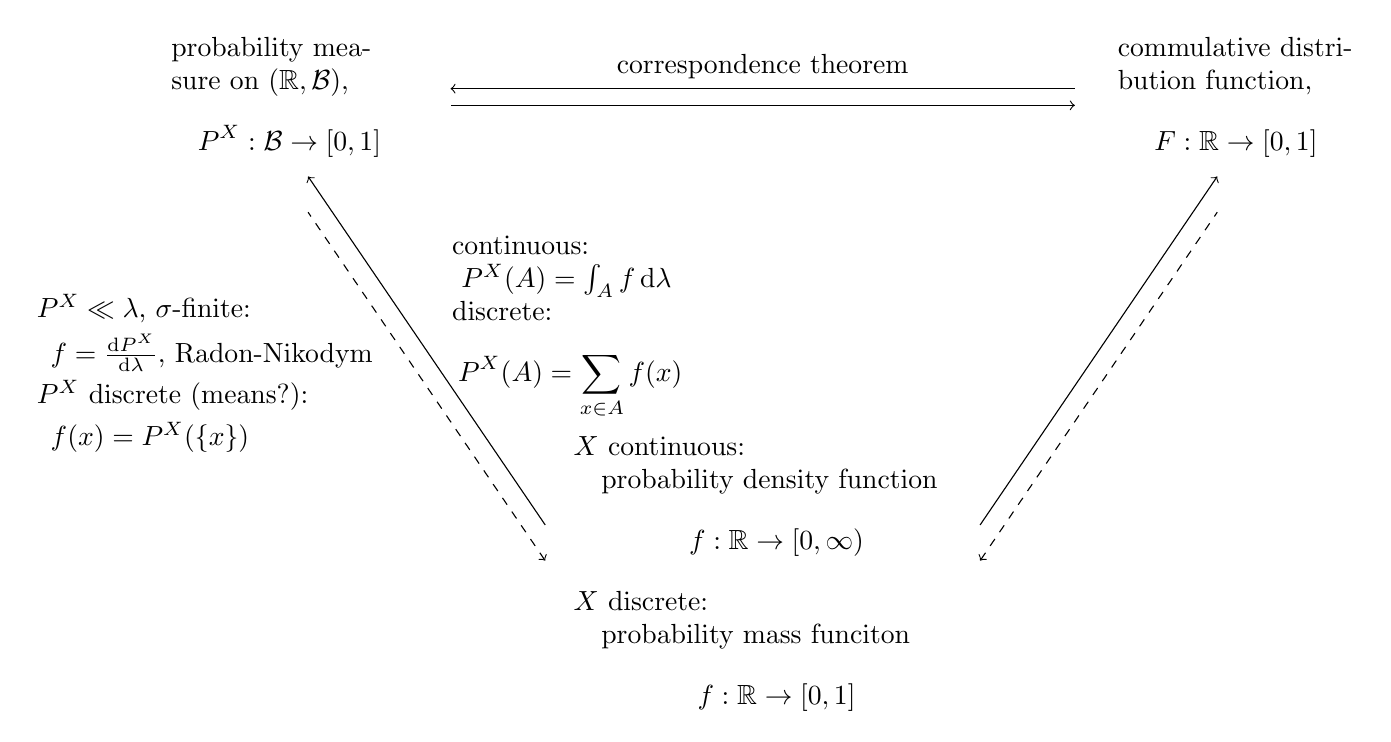
\begin{tikzpicture}[]
		\tikzstyle{equi} = [->,draw, shorten <=12pt, shorten >=12pt];
	
			\node (C) [text width=4.8cm, node distance = 6.5cm] {$X$ continuous: \\ \begin{addmargin}[1em]{0em} probability density function \[f: \mathbb{R} \to [0, \infty)\] \end{addmargin} $X$ discrete: \\ \begin{addmargin}[1em]{0em} probability mass funciton\[f:\mathbb{R} \to [0,1]\]\end{addmargin}};
  			\node (A) [above right of=C, text width=3cm, node distance = 8.5cm] {commulative distribution function, \[F: \mathbb{R} \to [0,1]\]};
  			\node (B) [above left of=C, text width=3cm, node distance = 8.5cm] {probability measure on $(\mathbb{R}, \mathcal{B})$, \[P^X: \mathcal{B} \to [0,1]\]};
  			
  			\tikzstyle{every path}=[equi]
		
			\draw[transform canvas={yshift=0.7ex},->] (A) -- node[anchor=west,above]{correspondence theorem} (B);  			
  			\draw[transform canvas={yshift=-0.7ex},<-] (A) --  (B);
  			\draw[transform canvas={yshift=1.5ex},<-] (B.270) -- node[right, text width=3cm, ,xshift=+0.2cm,yshift=0.3cm]{continuous:\\ $\, \, P^X(A) = \int_A f \,\mathrm{d}\lambda$\\discrete:\[P^X(A) = \sum_{x \in A} f(x)\]} (C.180);  			
  			\draw[transform canvas={yshift=-1.5ex},<-, dashed]  (C.180) -- node[below, text width=4.5cm, ,xshift=-2.7cm,yshift=1.3cm]{$P^X \ll \lambda$, $\sigma$-finite:\\ \smallskip $\,\,\,f=\frac{\mathrm{d}P^X}{\mathrm{d}\lambda}$, Radon-Nikodym\\ \smallskip $P^X$ discrete (means?):\\ \smallskip $\,\,\,f(x) = P^X(\{x\})$}  (B.270);
			\draw[transform canvas={yshift=1.5ex},<-] (A.270) --  node[above]{} (C.0);  			
  			\draw[transform canvas={yshift=-1.5ex},<-, dashed] (C.0) --  (A.270);

	
	\end{tikzpicture}
%}
\end{center}
   

\end{document}